\documentclass{ximera}
\graphicspath{  %% When looking for images,
{./}            %% look here first,
{./pictures/}   %% then look for a pictures folder,
{../pictures/}  %% which may be a directory up.
{../../pictures/}  %% which may be a directory up.
{../../../pictures/}  %% which may be a directory up.
{../../../../pictures/}  %% which may be a directory up.
}

\usepackage{listings}
\usepackage{circuitikz}
\usepackage{xcolor}
\usepackage{amsmath,amsthm}
\usepackage{subcaption}
\usepackage{graphicx}
\usepackage{tikz}
\usepackage{tikz-3dplot}
\usepackage{amsfonts}
\usepackage{mdframed} % For framing content
\usepackage{tikz-cd}

  \renewcommand{\vector}[1]{\left\langle #1\right\rangle}
  \newcommand{\arrowvec}[1]{{\overset{\rightharpoonup}{#1}}}
  \newcommand{\ro}{\texttt{R}}%% row operation
  \newcommand{\dotp}{\bullet}%% dot product
  \renewcommand{\l}{\ell}
  \let\defaultAnswerFormat\answerFormatBoxed
  \usetikzlibrary{calc,bending}
  \tikzset{>=stealth}
  




%make a maroon color
\definecolor{maroon}{RGB}{128,0,0}
%make a dark blue color
\definecolor{darkblue}{RGB}{0,0,139}
%define the color fourier0 to be the maroon color
\definecolor{fourier0}{RGB}{128,0,0}
%define the color fourier1 to be the dark blue color
\definecolor{fourier1}{RGB}{0,0,139}
%define the color fourier 1t to be the light blue color
\definecolor{fourier1t}{RGB}{173,216,230}
%define the color fourier2 to be the dark green color
\definecolor{fourier2}{RGB}{0,100,0}
%define teh color fourier2t to be the light green color
\definecolor{fourier2t}{RGB}{144,238,144}
%define the color fourier3 to be the dark purple color
\definecolor{fourier3}{RGB}{128,0,128}
%define the color fourier3t to be the light purple color
\definecolor{fourier3t}{RGB}{221,160,221}
%define the color fourier0t to be the red color
\definecolor{fourier0t}{RGB}{255,0,0}
%define the color fourier4 to be the orange color
\definecolor{fourier4}{RGB}{255,165,0}
%define the color fourier4t to be the darker orange color
\definecolor{fourier4t}{RGB}{255,215,0}
%define the color fourier5 to be the yellow color
\definecolor{fourier5}{RGB}{255,255,0}
%define the color fourier5t to be the darker yellow color
\definecolor{fourier5t}{RGB}{255,255,100}
%define the color fourier6 to be the green color
\definecolor{fourier6}{RGB}{0,128,0}
%define the color fourier6t to be the darker green color
\definecolor{fourier6t}{RGB}{0,255,0}

%New commands for this doc for errors in copying
\newcommand{\eigenvar}{\lambda}
%\newcommand{\vect}[1]{\mathbf{#1}}
\renewcommand{\th}{^{\text{th}}}
\newcommand{\st}{^{\text{st}}}
\newcommand{\nd}{^{\text{nd}}}
\newcommand{\rd}{^{\text{rd}}}
\newcommand{\paren}[1]{\left(#1\right)}
\newcommand{\abs}[1]{\left|#1\right|}
\newcommand{\R}{\mathbb{R}}
\newcommand{\C}{\mathbb{C}}
\newcommand{\Hilb}{\mathbb{H}}
\newcommand{\qq}[1]{\text{#1}}
\newcommand{\Z}{\mathbb{Z}}
\newcommand{\N}{\mathbb{N}}
\newcommand{\q}[1]{\text{``#1''}}
%\newcommand{\mat}[1]{\begin{bmatrix}#1\end{bmatrix}}
\newcommand{\rref}{\text{reduced row echelon form}}
\newcommand{\ef}{\text{echelon form}}
\newcommand{\ohm}{\Omega}
\newcommand{\volt}{\text{V}}
\newcommand{\amp}{\text{A}}
\newcommand{\Seq}{\textbf{Seq}}
\newcommand{\Poly}{\textbf{P}}
\renewcommand{\quad}{\text{    }}
\newcommand{\roweq}{\simeq}
\newcommand{\rowop}{\simeq}
\newcommand{\rowswap}{\leftrightarrow}
\newcommand{\Mat}{\textbf{M}}
\newcommand{\Func}{\textbf{Func}}
\newcommand{\Hw}{\textbf{Hamming weight}}
\newcommand{\Hd}{\textbf{Hamming distance}}
\newcommand{\rank}{\text{rank}}
\newcommand{\longvect}[1]{\overrightarrow{#1}}
% Define the circled command
\newcommand{\circled}[1]{%
  \tikz[baseline=(char.base)]{
    \node[shape=circle,draw,inner sep=2pt,red,fill=red!20,text=black] (char) {#1};}%
}

% Define custom command \strikeh that just puts red text on the 2nd argument
\newcommand{\strikeh}[2]{\textcolor{red}{#2}}

% Define custom command \strikev that just puts red text on the 2nd argument
\newcommand{\strikev}[2]{\textcolor{red}{#2}}

%more new commands for this doc for errors in copying
\newcommand{\SI}{\text{SI}}
\newcommand{\kg}{\text{kg}}
\newcommand{\m}{\text{m}}
\newcommand{\s}{\text{s}}
\newcommand{\norm}[1]{\left\|#1\right\|}
\newcommand{\col}{\text{col}}
\newcommand{\sspan}{\text{span}}
\newcommand{\proj}{\text{proj}}
\newcommand{\set}[1]{\left\{#1\right\}}
\newcommand{\degC}{^\circ\text{C}}
\newcommand{\centroid}[1]{\overline{#1}}
\newcommand{\dotprod}{\boldsymbol{\cdot}}
%\newcommand{\coord}[1]{\begin{bmatrix}#1\end{bmatrix}}
\newcommand{\iprod}[1]{\langle #1 \rangle}
\newcommand{\adjoint}{^{*}}
\newcommand{\conjugate}[1]{\overline{#1}}
\newcommand{\eigenvarA}{\lambda}
\newcommand{\eigenvarB}{\mu}
\newcommand{\orth}{\perp}
\newcommand{\bigbracket}[1]{\left[#1\right]}
\newcommand{\textiff}{\text{ if and only if }}
\newcommand{\adj}{\text{adj}}
\newcommand{\ijth}{\emph{ij}^\text{th}}
\newcommand{\minor}[2]{M_{#2}}
\newcommand{\cofactor}{\text{C}}
\newcommand{\shift}{\textbf{shift}}
\newcommand{\startmat}[1]{
  \left[\begin{array}{#1}
}
\newcommand{\stopmat}{\end{array}\right]}
%a command to give a name to explorations and hints and theorems
\newcommand{\name}[1]{\begin{centering}\textbf{#1}\end{centering}}
\newcommand{\vect}[1]{\vec{#1}}
\newcommand{\dfn}[1]{\textbf{#1}}
\newcommand{\transpose}{\mathsf{T}}
\newcommand{\mtlb}[2][black]{\texttt{\textcolor{#1}{#2}}}
\newcommand{\RR}{\mathbb{R}} % Real numbers
\newcommand{\id}{\text{id}}

\author{Zack Reed}
\begin{document}

%matrix_sum_and_diff
\begin{problem}
  For the following pairs of matrices, does the sum $A+B$ and difference $A-B$ make sense? (i.e. is an element-by-element calculation possible?) If so, calculate them.
  \begin{enumerate}
  \item
    $A = \begin{mymatrix}{rr}
      1 & 0 \\
      0 & 1
    \end{mymatrix}$,\quad
    $B = \begin{mymatrix}{rr}
      0 & 1 \\
      1 & 0
    \end{mymatrix}$.

    \begin{sol}
    

      $A+B$ and $A-B$ $\answer{\text{are}}$ possible because 

      \begin{selectAll}
        \choice[correct]{they have the same dimensions}
        \choice{they have different dimensions}
        \choice{each element of $A$ cannot be matched with any element of $B$}
        \choice[correct]{each element of $A$ can be matched with an element of $B$ in the same location}
        \choice{elements of $A$ cannot be matched with elements of $B$ in the same location and vice versa}
      \end{selectAll}

      $A+B = \begin{mymatrix}{rr}
        \answer{1} & \answer{1} \\
        \answer{1} & \answer{1}
      \end{mymatrix}$,\quad

      $A-B = \begin{mymatrix}{rr}
        \answer{1} & \answer{-1} \\
        \answer{-1} & \answer{1}
      \end{mymatrix}$.


    \end{sol}

  \item
    $A = \begin{mymatrix}{rrr}
      2 & 1 & 2 \\
      1 & 1 & 0
    \end{mymatrix}$,\quad
    $B = \begin{mymatrix}{rrr}
      -1 & 0 & 3 \\
      0 & 1 & 4
    \end{mymatrix}$.

    \begin{sol}
    

      $A+B$ and $A-B$ $\answer{\text{are}}$ possible because 

      \begin{selectAll}
        \choice[correct]{they have the same dimensions}
        \choice{they have different dimensions}
        \choice{each element of $A$ cannot be matched with any element of $B$}
        \choice[correct]{each element of $A$ can be matched with an element of $B$ in the same location}
        \choice{elements of $A$ cannot be matched with elements of $B$ in the same location and vice versa}
      \end{selectAll}

      $A+B = \begin{mymatrix}{rrr}
        \answer{1} & \answer{1} & \answer{5} \\
        \answer{1} & \answer{2} & \answer{4}
      \end{mymatrix}$,\quad

      $A-B = \begin{mymatrix}{rrr}
        \answer{3} & \answer{1} & \answer{-1} \\
        \answer{1} & \answer{0} & \answer{-4}
      \end{mymatrix}$.
      \end{sol}

  \item
    $A = \begin{mymatrix}{rr}
      1 & 0 \\
      -2 & 3 \\
      4 & 2
    \end{mymatrix}$,\quad
    $B = \begin{mymatrix}{rrr}
      2 & 7 & -1 \\
      0 & 3 & 4
    \end{mymatrix}$.


    \begin{sol}
    

      $A+B$ and $A-B$ $\answer{\text{are not}}$ possible because 

      \begin{selectAll}
        \choice{they have the same dimensions}
        \choice[correct]{they have different dimensions}
        \choice{each element of $A$ cannot be matched with any element of $B$}
        \choice{each element of $A$ can be matched with an element of $B$ in the same location}
        \choice[correct]{elements of $A$ cannot be matched with elements of $B$ in the same location and vice versa}
      \end{selectAll}
      
      %MAKE THIS HIDDEN TILL THEY ANSWER THE PREVIOUS ONE
      If we instead took $B^T$, then $A+B^T$ and $A-B^T$ would be possible.

      $A+B^T = \begin{mymatrix}{rr}
        \answer{0} & \answer{4}  \\
        \answer{5} & \answer{6}  \\
        \answer{6} & \answer{2} 
      \end{mymatrix}$,\quad

      $A-B^T = \begin{mymatrix}{rr}
        \answer{2} & \answer{-4}  \\
        \answer{-9} & \answer{0}  \\
        \answer{2} & \answer{2} 
      \end{mymatrix}$.



      \end{sol}

  \end{enumerate}
\end{problem}

%matrix_neg_and_transpose
\begin{problem}
  For each matrix $A$, find the matrix $-A$ and $A^T$.
  \begin{enumerate}
  \item
    $A = \begin{mymatrix}{rr}
      1 & 2 \\
      2 & 1
    \end{mymatrix}$

  \item
    $A = \begin{mymatrix}{rr}
      -2 & 3 \\
      0 & 2
    \end{mymatrix}$

  \item
    $A = \begin{mymatrix}{rrr}
      0 & 1 & 2 \\
      1 & -1 & 3 \\
      4 & 2 & 0
    \end{mymatrix}$
  \end{enumerate}
  % \begin{sol}
  % \end{sol}
\end{problem}

%matrix_linear_combinations
\begin{problem}

  For each group of matrices and each group of scalars, find the linear combination.

  \begin{enumerate}
  \item
    $A = \begin{mymatrix}{rr}
      1 & 2 \\
      2 & 1
    \end{mymatrix}$,\quad
    $B = \begin{mymatrix}{rr}
      0 & 1 \\
      1 & 0
    \end{mymatrix}$,\quad
    $C = \begin{mymatrix}{rr}
      1 & 0 \\
      0 & 1
    \end{mymatrix}$,\quad
    $a = 2$, $b = -1$, $c = 3$.

    $aA + bB + cC = \begin{mymatrix}{rr}
      \answer{5} & \answer{3} \\
      \answer{3} & \answer{5}
    \end{mymatrix}$.

  \item 
    $A = \begin{mymatrix}{rrrr}
      1 & 2 & 5 & 4 \\
      2 & 0 & 3 & 1
    \end{mymatrix}$,\quad
    $B = \begin{mymatrix}{rrrr}
      0 & 3 & 1 & 2 \\
      10 & 8 & 0 & 1
    \end{mymatrix}$,\quad
    $C = \begin{mymatrix}{rrrr}
      10 & 6 & 2 & 3 \\
      1 & 4 & 7 & 3
    \end{mymatrix}$,\quad
    $a = 3$, $b = -2$, $c = 4$.

    \begin{hint}

      Arithmetic in MATLAB will make this easier. For example, if you define $A$, $B$, and $C$ as matrices and then $a$, $b$, and $c$ as scalars, you can calculate the linear combination with the command $a*A + b*B + c*C$.

    \end{hint}

    $aA + bB + cC = \begin{mymatrix}{rrrr}
      \answer{43} & \answer{24} & \answer{21} & \answer{20} \\
      \answer{-10} & \answer{0} & \answer{37} & \answer{13}
    \end{mymatrix}$.

  \end{enumerate}

\end{problem}

%matrix_algebra
\begin{problem}
  Let $A = \begin{mymatrix}{rrr}
    1 & 2 & -1 \\
    -1 & 4 & 0 \\
  \end{mymatrix}$ and
  $B = \begin{mymatrix}{rrr}
    0 & 3 & 0 \\
    1 & -1 & 1 \\
  \end{mymatrix}$.\par\noindent
  Find a matrix $X$ such that $(A+X)-(B+0) = B+A$. 
  
  \begin{hint}
    First simplify the matrix equation using properties of matrix addition and scaling, then solve for $X$ using the matrices $A$ and $B$.
  \end{hint}

  \begin{sol}
    The equation simplifies to $X=B+B=2B$, so $X = \begin{mymatrix}{rrr}
    0 & 6 & 0 \\
    2 & -2 & 2 \\
    \end{mymatrix}$.
  \end{sol}
\end{problem}

%matrix_equality
\begin{problem}
  Find scalars $x,y,z$ such that the following two matrices are equal.
  \begin{equation*}
    \begin{mymatrix}{rr}
      x & -1 \\
      2 & 4
    \end{mymatrix}
    \quad\mbox{and}\quad
    \begin{mymatrix}{rr}
      2 & y \\
      z & 4
    \end{mymatrix}.
  \end{equation*}
  \begin{sol}
    $x=\answer{2}$, $y=\answer{-1}$, $z=\answer{2}$.
  \end{sol}
\end{problem}

%matrix_dimensions
\begin{problem}
  What are the dimensions of the following matrices?
  \begin{equation*}
    A = \begin{mymatrix}{rrr}
      1 & -2 & 0 \\
      4 & 3 & 2
    \end{mymatrix},
    \quad
    B = \begin{mymatrix}{rrr}
      3 & 4 & 1 \\
      1 & 3 & 1 \\
      6 & 2 & 2
    \end{mymatrix},
    \quad
    C = \begin{mymatrix}{rrr}
      1 & 0 \\
      4 & 0 \\
      2 & 0 \\
      0 & 0
    \end{mymatrix}.
  \end{equation*}
  \begin{sol}
    $A$ has dimensions $\answer{2}\times \answer{3}$, $B$ has dimensions $\answer{3}\times \answer{3}$, and C has dimensions ${4}\times {2}$.
  \end{sol}
\end{problem}

%big_matrix_entries
\begin{problem}
  What is the $(2,3)$-entry of the matrix $A=\begin{mymatrix}{rrr}
    1 & 2 & 1 \\
    -4 & 4 & 7 \\
    6 & -5 & 3
  \end{mymatrix}$?
  \begin{sol}
    $A(2,3)=\answer{7}$.
  \end{sol}

  What is the $(17,8)$ entry of $A$, the $(2,22)$ entry of $A^T$, and the $(29,8)$ entry of $30A$, where $A$ is given in the hint below. 
  
  You will want to copy the matrix directly into MATLAB and then use MATLAB to find the answers.

  \begin{hint}

    A=[
  0.3567, 0.7912, 0.6215, 0.4321, 0.9998, 0.2837, 0.5124, 0.6185, 0.7345, 0.2789;
  0.8941, 0.4725, 0.5293, 0.1268, 0.8556, 0.1423, 0.6789, 0.9143, 0.2278, 0.4502;
  0.1427, 0.9376, 0.8153, 0.3549, 0.5123, 0.6712, 0.4296, 0.7035, 0.8927, 0.6598;
  0.7289, 0.1856, 0.4632, 0.7462, 0.3924, 0.8741, 0.1532, 0.5824, 0.3619, 0.5431;
  0.2983, 0.5197, 0.9324, 0.2871, 0.7812, 0.1239, 0.8175, 0.2649, 0.4578, 0.6894;
  0.6378, 0.2413, 0.7496, 0.5631, 0.4298, 0.8179, 0.9342, 0.7823, 0.5147, 0.3705;
  0.4217, 0.6649, 0.2974, 0.8753, 0.5823, 0.4912, 0.7326, 0.6814, 0.2913, 0.8476;
  0.9135, 0.3547, 0.5842, 0.1263, 0.4593, 0.2834, 0.7291, 0.9402, 0.1753, 0.5128;
  0.7392, 0.4826, 0.2154, 0.8972, 0.6938, 0.3481, 0.6415, 0.5143, 0.7923, 0.2345;
  0.5834, 0.7421, 0.3148, 0.6259, 0.3981, 0.9762, 0.5178, 0.3827, 0.6845, 0.4192;
  0.4912, 0.3746, 0.8159, 0.2541, 0.7639, 0.6318, 0.1925, 0.8593, 0.6248, 0.7352;
  0.8297, 0.4562, 0.3718, 0.5794, 0.2643, 0.7129, 0.8943, 0.4872, 0.3126, 0.9614;
  0.6751, 0.5239, 0.7485, 0.3917, 0.8126, 0.2671, 0.9352, 0.7145, 0.5798, 0.1467;
  0.3198, 0.8271, 0.2463, 0.4862, 0.7382, 0.6457, 0.9213, 0.2689, 0.4982, 0.8543;
  0.4825, 0.6914, 0.5428, 0.3769, 0.2581, 0.7385, 0.6174, 0.9583, 0.8312, 0.3459;
  0.2471, 0.8342, 0.1265, 0.6934, 0.5216, 0.3978, 0.7489, 0.6597, 0.2843, 0.8715;
  0.6438, 0.3197, 0.5876, 0.7548, 0.3945, 0.8274, 0.6317, 0.5482, 0.9537, 0.2184;
  0.7384, 0.4715, 0.9362, 0.1683, 0.5197, 0.2734, 0.4817, 0.8492, 0.6253, 0.7648;
  0.9267, 0.3125, 0.8549, 0.3972, 0.6718, 0.4239, 0.9125, 0.3874, 0.5246, 0.6923;
  0.3745, 0.6193, 0.4897, 0.8624, 0.2497, 0.7318, 0.5463, 0.8394, 0.2371, 0.4978;
  0.5378, 0.7129, 0.3287, 0.8652, 0.4321, 0.9487, 0.2735, 0.6142, 0.5839, 0.7516;
    0.6219, 0.3498, 0.4867, 0.7824, 0.5472, 0.6314, 0.9271, 0.4578, 0.7912, 0.6384;
    0.7693, 0.4852, 0.6428, 0.3196, 0.8327, 0.4129, 0.7692, 0.5628, 0.6917, 0.4735;
    0.8257, 0.5738, 0.3471, 0.4963, 0.7892, 0.2187, 0.8571, 0.6294, 0.4158, 0.8627;
    0.3985, 0.7283, 0.5824, 0.6731, 0.5186, 0.6297, 0.4576, 0.8924, 0.2639, 0.5487;
    0.5479, 0.6894, 0.2137, 0.7846, 0.4517, 0.7694, 0.8325, 0.3672, 0.6398, 0.7325;
    0.8375, 0.6128, 0.4783, 0.5297, 0.6921, 0.8219, 0.3478, 0.7184, 0.6273, 0.4931;
    0.4961, 0.7842, 0.5374, 0.6829, 0.2485, 0.5617, 0.7293, 0.3982, 0.6194, 0.8123;
    0.7138, 0.3584, 0.7914, 0.4126, 0.5932, 0.6418, 0.3784, 0.7493, 0.8176, 0.2589;
    0.6527, 0.2947, 0.8193, 0.6318, 0.4938, 0.5672, 0.2387, 0.7962, 0.5214, 0.6849
];

  \end{hint}

$A(17,8)=\answer{0.5482}$, $A^T(2,22)=\answer{0.3498}$, and $30A(29,8)=\answer{22.4790}$.

\end{problem}

%matrix_products
\begin{problem}
  For each matrix $A$, find the products $(-2)A$, $0A$, and $512A$.
  \begin{enumerate}
  \item
    $A = \begin{mymatrix}{rr}
      1 & 2 \\
      2 & 1
    \end{mymatrix}$
  \item
    $A = \begin{mymatrix}{rr}
      -2 & 3 \\
      0 & 2
    \end{mymatrix}$
  \item
    $A = \begin{mymatrix}{rrr}
      0 & 1 & 2 \\
      1 & -1 & 3 \\
      4 & 2 & 0
    \end{mymatrix}$
  \end{enumerate}
  % \begin{sol}
  % \end{sol}
\end{problem}

%matrix_symmetry
\begin{problem}
  Consider the matrices
  \begin{equation*}
    A =\begin{mymatrix}{rr}
      1 & 2 \\
      3 & 2 \\
      1 & -1
    \end{mymatrix},
    \quad
    B=\begin{mymatrix}{rrr}
      2 & -5 & 2 \\
      -3 & 2 & 1
    \end{mymatrix}
  \end{equation*}
  Find the following if possible. If it is not possible explain why.
  \begin{enumerate}
  \item $-3A{^T}$.
  \item $3B - A^T$.
  \end{enumerate}

  \begin{sol}
    \begin{enumerate}
    \item $\begin{mymatrix}{rrr}
        -3 & -9 & -3 \\
        -6 & -6 & 3
      \end{mymatrix}$.
    \item $\begin{mymatrix}{rrr}
        5 & -18 & 5 \\
        -11 & 4 & 4
      \end{mymatrix}$.
    \end{enumerate}
  \end{sol}

  Which of the following matrices are symmetric, antisymmetric, both,
  or neither?
  \begin{equation*}
    A = \begin{mymatrix}{rr}
      0 & 1 \\
      -1 & 0 \\
    \end{mymatrix},
    \quad
    B = \begin{mymatrix}{rr}
      2 & 1 \\
      1 & 3 \\
    \end{mymatrix},
    \quad
    C = \begin{mymatrix}{rr}
      1 & 2 \\
      -2 & 0 \\
    \end{mymatrix},
    \quad
    D = \begin{mymatrix}{rr}
      0 & 0 \\
      0 & 0 \\
    \end{mymatrix}.
  \end{equation*}
  \begin{sol}
    $A$ is antisymmetric, $B$ is symmetric, $C$ is neither, and $D$ is both.
  \end{sol}
\end{problem}

%images_as_matrices
\begin{problem}

%Show images as the transpose of matrices using includegraphics on test_image.jpg

Suppose that the matrix $A$ gives the grayscale values of the following image of a lion:

\begin{figure}[h]
  \centering
  \begin{subfigure}[b]{0.45\textwidth}
    \centering
    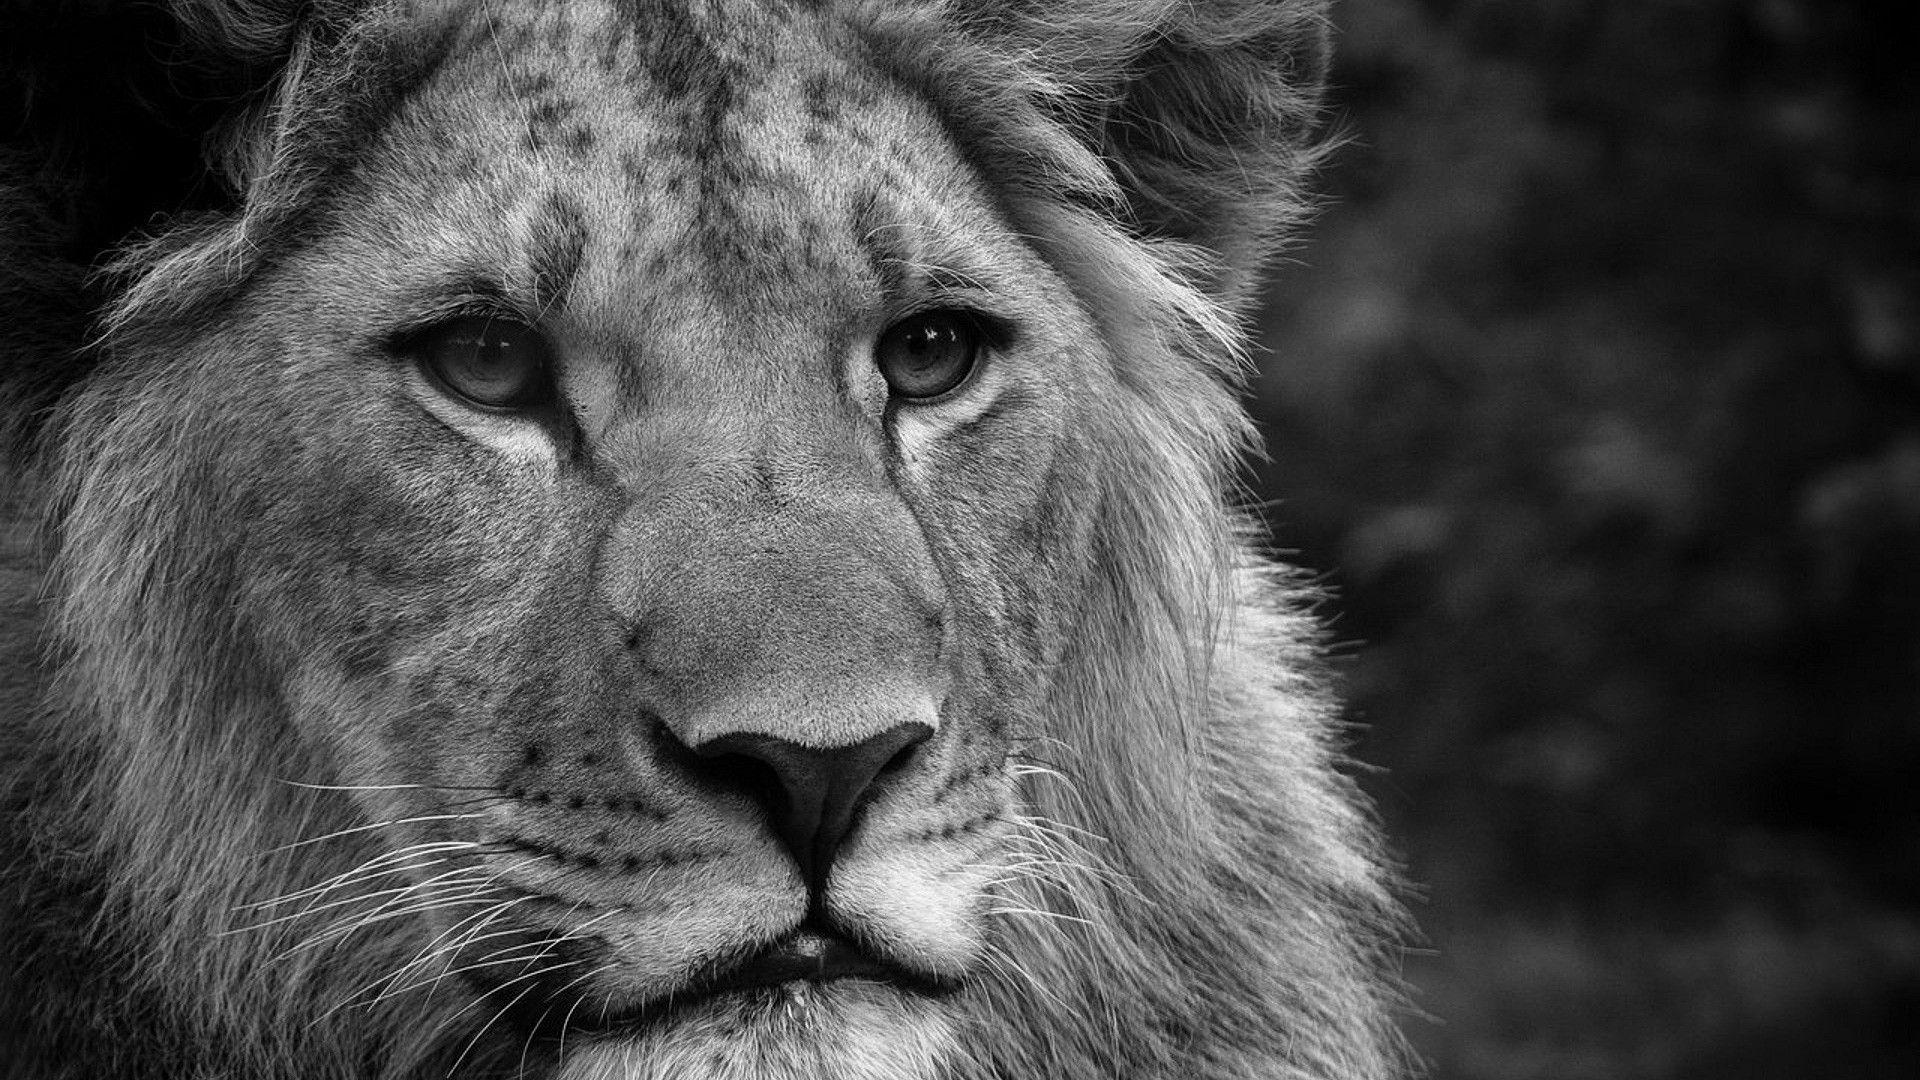
\includegraphics[width=\textwidth]{test_image.jpg}
    \caption{Original Image}
    \label{fig:original}
  \end{subfigure}
  \hfill
  \begin{subfigure}[b]{0.45\textwidth}
    \centering
    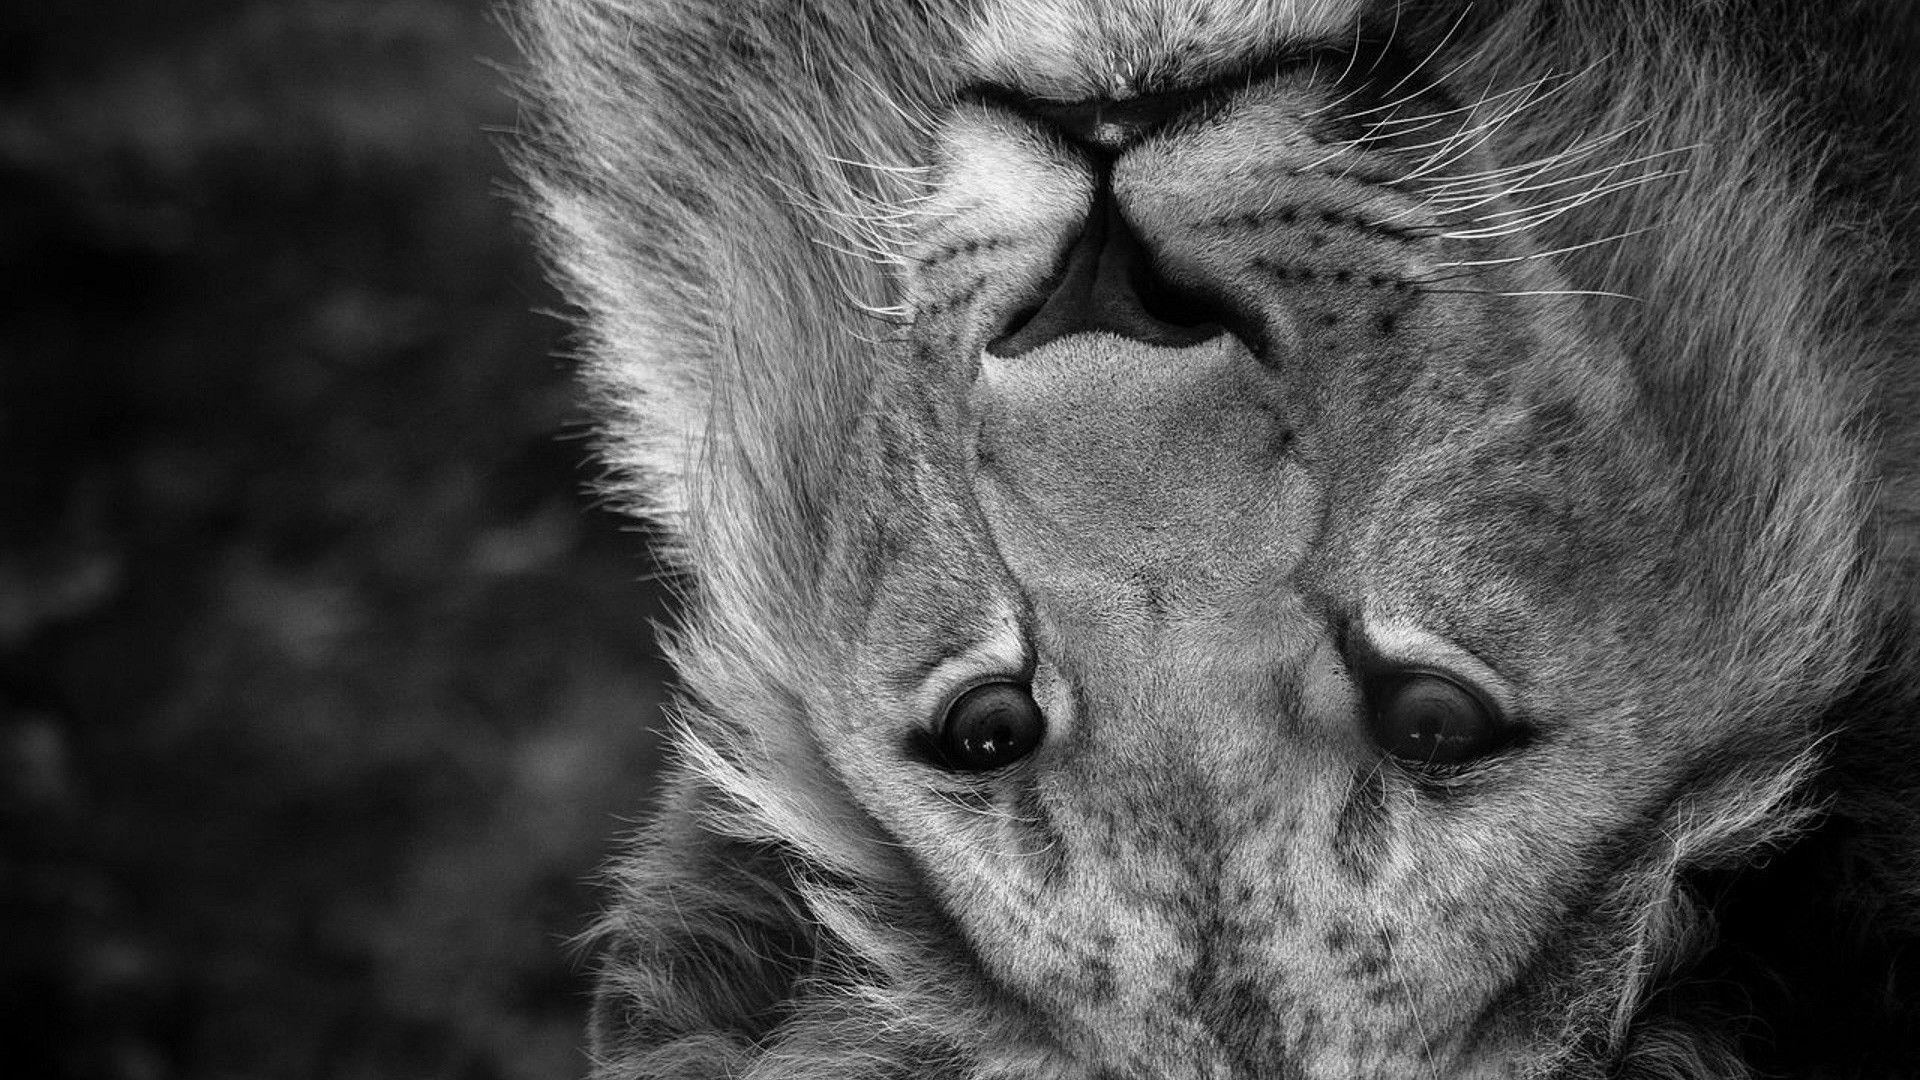
\includegraphics[width=\textwidth]{test_image_rot_2.jpg}
    \caption{Option A}
    \label{fig:optionA}
  \end{subfigure}
\end{figure}

\begin{figure}[h]
  \centering
  \begin{subfigure}[b]{0.35\textwidth}
    \centering
    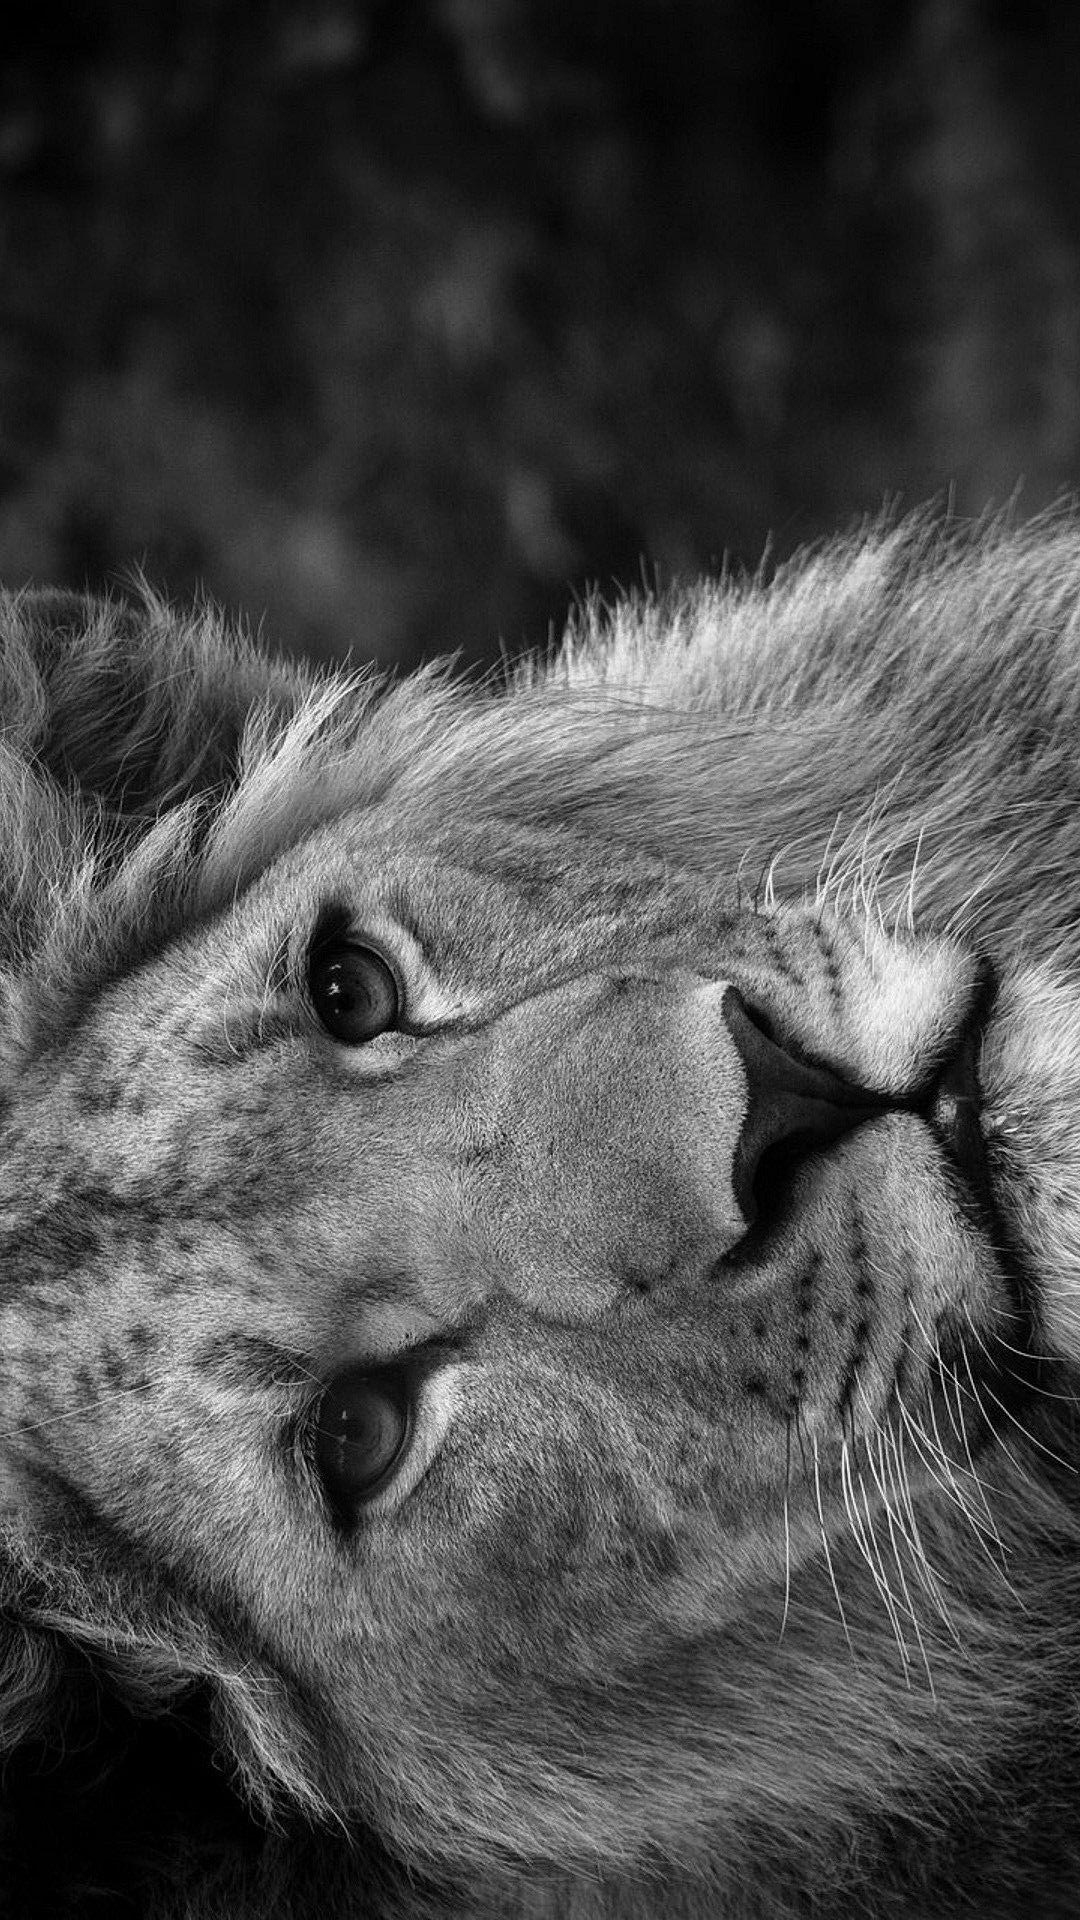
\includegraphics[width=\textwidth]{test_image_rot_1.jpg}
    \caption{Option C}
    \label{fig:optionC}
  \end{subfigure}
  \hfill
  \begin{subfigure}[b]{0.35\textwidth}
    \centering
    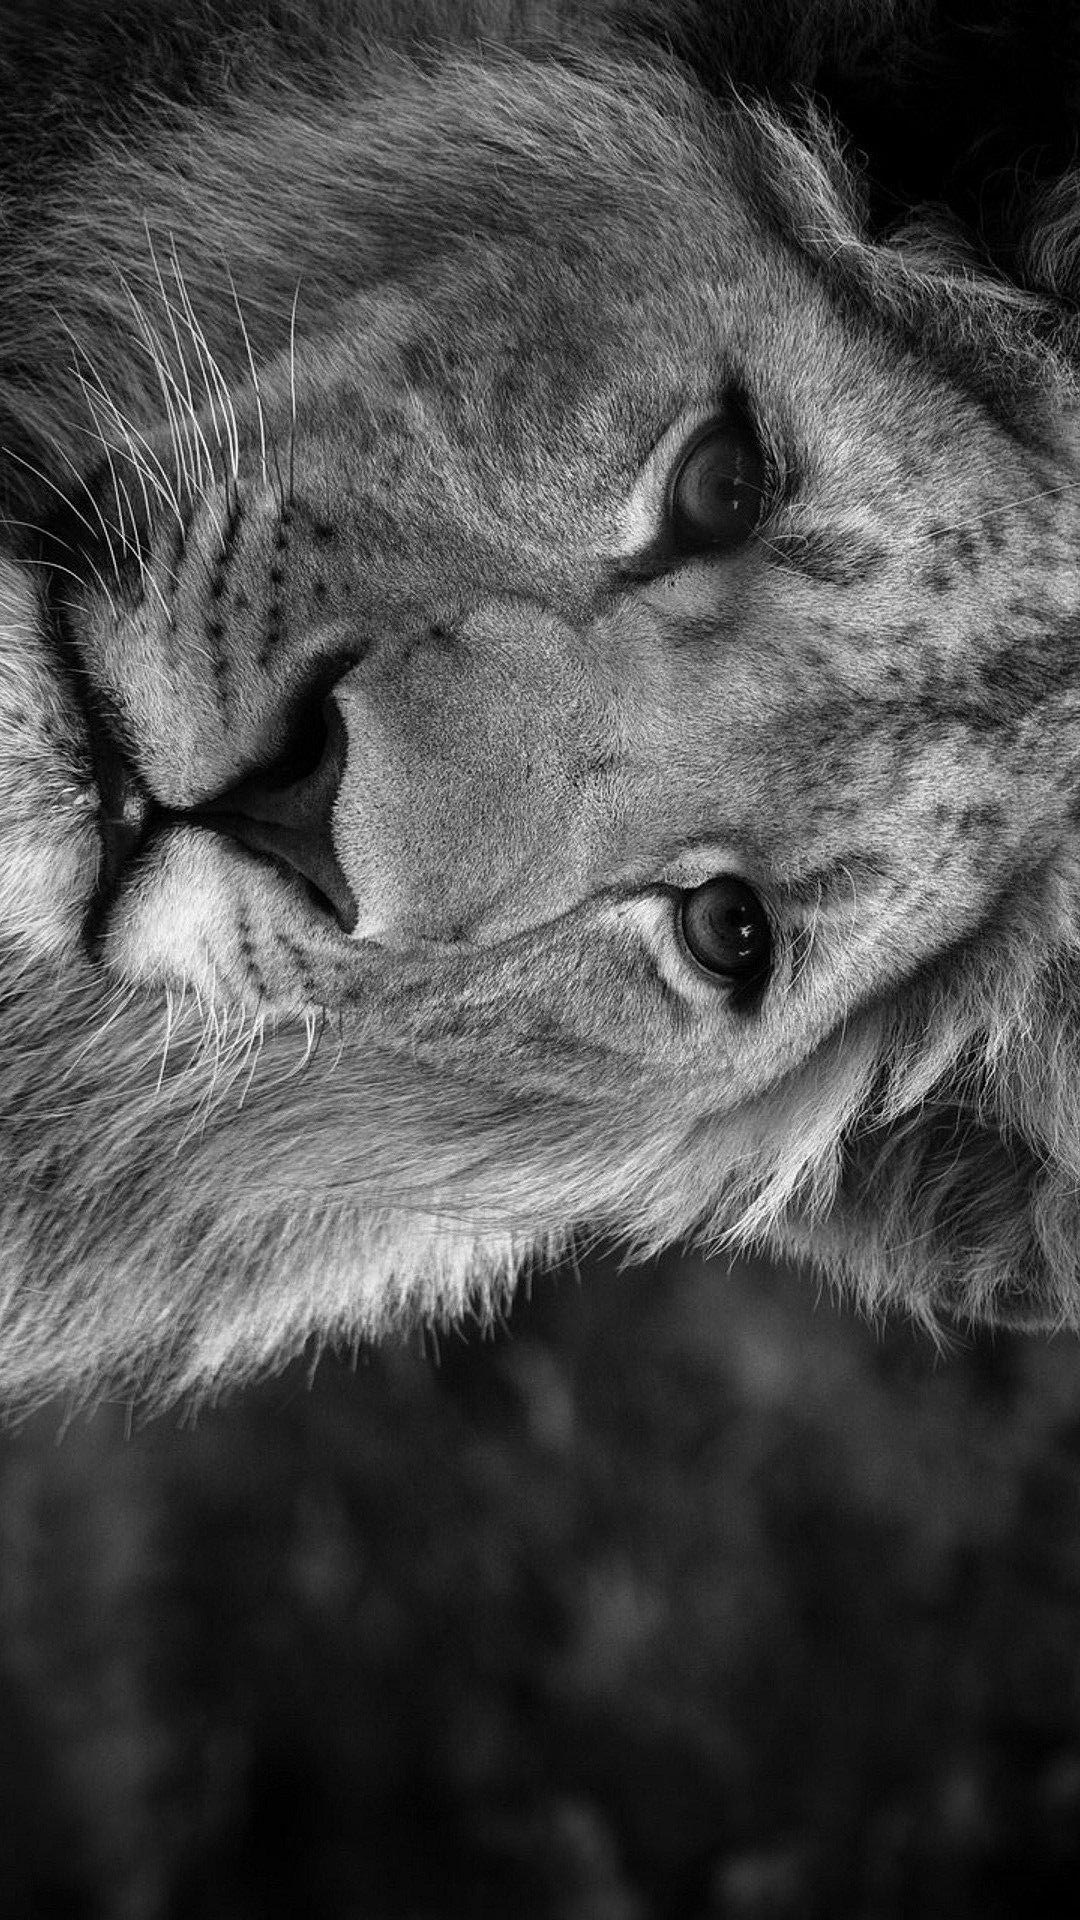
\includegraphics[width=\textwidth]{test_image_rot_3.jpg}
    \caption{Option D}
    \label{fig:optionD}
  \end{subfigure}
\end{figure}

Which image(s) below correspond to $A^T$? (Select all that apply)

\begin{selectAll}

  \choice{Option A}
  \choice{Option B}
  \choice[correct]{Option C}
  \choice{Option D}

\end{selectAll}

Which image(s) below correspond to $(A^T)^T$? (Select all that apply)

\begin{selectAll}

  \choice[correct]{Option A}
  \choice{Option B}
  \choice{Option C}
  \choice{Option D}

\end{selectAll}


\end{problem}


\end{document}